% !TEX root=/home/tavant/these/manuscript/src/manuscript.tex




\chapter{Axial Azimuthal 2D PIC simulation}
\label{ch-5}

\headerchaptername{Axial Azimuthal 2D PIC simulation}

\inlinenote{Because I added this chapter, maybe the Z-theta code must be introduced in Ch-1.}
\begin{Chabstract}
  We modify the simulation code \LPPic in order to simulate the Axial-azimuthal simulation plan.
  This allows to confront the conclusion obtained from the results of the radial-azimuthal.
  In particular the impact of the electron diamagnetic drift and the axial transport of the instability.
  
  The impact of the radial plasma-wall interaction is also studied, and the question of the radial heating is discussed. 
\end{Chabstract}

% 
% 
% {\bf V. analyse of the instability } 30 pages
% \begin{zzz}
%   \begin{itemize}
% \item Instability dispersion relation
% \item Kinetic solver for Ion and ECDI using VDFs
% \item Impact of the difference w/r Maxwellian
% \item Wall Boundary condition, 3D dispertion relation vs 1D and 2D relations
% \item Linear stage as ECDI and Saturation toward IAW
% \end{itemize}
% \end{zzz}

\minitoc


% !TEX root=/home/tavant/these/manuscript/src/manuscript.tex

\section{Presentation of the Axial-azimuthal simulation}

The objectives of the axial-azimuthal simulation is to allows the azimuthal \ac{ECDI} to grow and study the impacts of the axial direction.
These impacts are mostly due to the radial magnetic field  that present a maximum close to the exit plane.

\subsection{Description of the simulation domaine} \label{subsec-ztheta_description}
\Cref{fig-3Dschematic} shows the simplified \ac{HET} annular channel with both the radial-azimuthal and the axial-azimuthal \ztheta domain.

\begin{figure}[hbt]
  \centering
  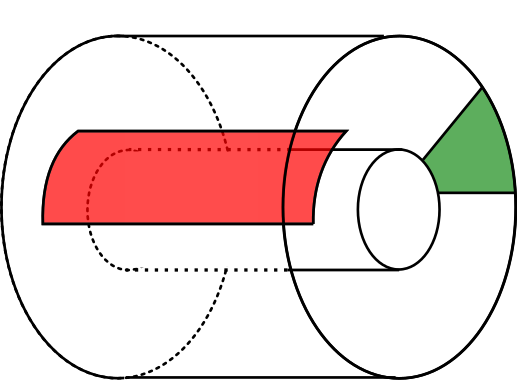
\includegraphics[width=0.6\textwidth]{3D_shematic}
  \caption{Schematic representation of the chamber of a \ac{HET} and (green) the Radial-azimuthal and (red) the axial-azimuthal 2D simulation domains.}
  \label{fig-3Dschematic}
\end{figure}

The \ac{2D} \ztheta domain is located at the mean radius of the channel, but its curvature is neglected.
\Cref{fig-2D_ztheta_bis} presents a schematic representation of the \ztheta simulation domain.
The anode side is closed by a metallic fully absorbing electrode, with a fixed non-zero potential.
On the other side of the domain, the near-plume region (a few centimetres from the exit plane) is modeled.
The boundary located in the near-plume is also a Dirichlet boundary condition, this time grounded.
The azimuthal direction is closed with periodic boundaries for both the particles and the fields.

\begin{figure}[hbt]
  \centering
  \includegraphics[width=0.6\textwidth]{2D_ztheta}
  \caption{Schematic representation of the \ac{2D} \ztheta simulation domain.}
  \label{fig-2D_ztheta_bis}
\end{figure}

The axial and azimuthal electric fields are self-consistently computed from the charge density by solving the Poisson equation.
Consequently, the simulation domain is not so different from the radial-azimuthal simulation domain.
This has allow us to adapt the code \LPPic to simulate both domain.

Two particular aspects have been developed\string: the cathode electron emission and the dynamic computational load balancing.

\paragraph{Cathode electron emission\\}
The cathode used in electrical propulsion are mostly used to neutralize the ion beam, but a significant fraction of the emitted elections enters the channel and travels toward the anode.
The electrons are injected at (or close to) the cathode boundary following a Maxwellian distribution of a few electron volts.
The number of electrons to inject at each time step is computed by closing the eternal circuit between the anode and the cathode.

In the real set-up, an electric filter is placed between the thruster and the generator \citep{barral2008}, originally placed to protect the power supply against AC current.
While this external circuit can be modeled \citep{verboncoeur1993}, and is susceptible to impact the thruster behavior \citep{barral2008,wei2017}, we neglect it in this study for sake of clarity.
Thus, the cathode current equals the anode current \[ I_a = I_c. \]
The corresponding number of electron to inject in the simulation domain depends whether the electron are injected at the boundary or in the domain. 
Therefore, they are developed in the next section.

\paragraph{Dynamic computational load balancing\\}
The axial profile of the plasma density presents a maximum that can be one order of magnitude higher than the mean plasma density.
Consequently, a static MPI domain decomposition would produce an unbalance in the number of numerical particle per CPU, which results in an under-efficient code.

One possibility is to modify dynamically the weigh of the numerical particle relative to the plasma density, in order to keep a relatively constant number of particle per cell.
This can be done by fissioning (merging) the particles when they are too small, or by slitting them in smaller particles when they are too big \citep{shon2001,teunissen2014}.
However, such algorithm can modify the charge, momentum, or the energy of the system if not done carefully.
In \citet{vranic2015}, the authors present an algorithm to  conserve these quantities.
However, we chose not to implement it because of its error-prone complexity.

Instead, we implemented a dynamic redistribution of the CPU domain, so that every CPU own approximately the same number of particle.
As the density gradient is in the axial direction, we only change the axial size of the CPU domains.



\subsection{Facing the breathing mode} \label{subsec-breathmod}
The breathing mode comes from the coupling between the neutral gas flow and the plasma dynamics, via the ionization.
Under the typical conditions of the \ac{HET}, we observed this oscillation with a slows frequency, around  $10-30$ kHz, and a large amplitude, as the plasma density can change up to one order of magnitude during the oscillation period \citep{barral2003a,barral2009}.
This oscillation is much slower than the \ac{ECDI}, and is present in the totality of the channel.

If these oscillations are not problematic for the fluid or \ac{DK} simulations, they are for \ac{PIC} simulations.
Indeed, the total number of numerical particles is proportional to the plasma density, and a minimal number of particles is required to limit the numerical heating \citep{turner2006}.
Thus, when the mean plasma density oscillates, the number of numerical particles (hence the amount of memory used) can change drastically.
This reduces significantly the performance of the simulation code, and can lead to memory overflow if the memory available is not high enough to store all of the particles during the peak of density  of the oscillation.
The \emph{merging-splitting} of the particles  can be used to reduce the variation of the number of numerical particles, but it is not used for the same reason than discussed above.

In addition to the number of particles, the numerical parameters (time step and cell size) have to be chosen to satisfy the stability criteria during all of the simulation, which also reduces significantly the performance of the simulation. 
This could be overcome by adapting dynamically the mesh and the time step.
However, too few studies of the consequences of the use of merging-splitting and adaptive mesh on the simulation results have been conducted.
Thus, we have chosen not to modify the \ac{PIC} algorithm.


Two other approaches have been followed to reduce the computational cost of the breathing mode\string:
\begin{enumerate}
  \item the approach used by \citet{coche2014}\string: using a scaling of the permittivity to reduce the computational load,
  \item the approach of \citet{boeuf2017}, using a forced ionization source term.
\end{enumerate} 
These two cases are significantly different in the physics modeled and the behavior observed.
Hence, we will study both of them.

\subsection{Simulation test-case of Coche} \label{subsec-coche_description}

The simulation proposed by \citet{coche2014} models self-consistently the ionization with the \ac{MCC} algorithm, as well as the neutral gas flow.
\Cref{fig-coche-presnetation} presents the domain of simulation.
The simulation domain geometry is realistic, with a channel length $L_{channel} = 2.5\,\centi\meter$ for a total axial length of the simulation domain $L_z=4\,\centi\meter$.
Hence, the totality of the chamber and a part of the near plume is simulated.

 \renewcommand\subfigurewidth{0.4\textwidth}


\begin{figure}[hbt]
  \centering
  \begin{tabular}{cc}
    \subfigure{coches_domain}{}{10,10} &
    \subfigure{coches_profiles}{}{10,10} \\
  \end{tabular}
  \caption{(left) the \ac{2D} axial azimuthal domain; (right) the axial profile of the magnetic field and the initial xenon neutral gas profile used for the simulation case of Coche. }
  \label{fig-coche-presnetation}
\end{figure}


The neutral xenon is modeled by solving a system of \ac{1D} fluid equations.
Indeed, the azimuthal variations of the neutrals are neglected in this section.
The gas is modeled using the continuity and the momentum conservation equations\string:
\begin{align}
  \deriv{n_g}{t} &+ \deriv{(n_g v_g)}{z} = - S_{iz} \\
  \deriv{(n_g v_g)}{t} &+ \deriv{(n_g v_g^2)}{z} +  2 \deriv{( n_g D_g)}{z} = - S_{iz} v_g
\end{align}

with $n_g$ and $v_g$ the neutral gas density and axial velocity, respectively, $S_{iz}$ is the ionization source term obtained by the \ac{MCC} algorithm, and $D_n$ is used to close the system, and is \citep{coche2013}
\begin{equation} \label{eq-Dn}
  D_n = \frac{k_B T_g}{6 m_i}.
\end{equation}
The gas temperature $T_g=640K$ and the initial condition is described on the density $n_g$ on \cref{fig-coche-presnetation}(right).
The initial velocity is $v_g=200\,\meter\per\second$.


The constraints on the time step and the cell size are alleviated by using a scaling on the permittivity.
It is simply increased by a coefficient $\alpha$, as used in other low-temperature modelling \citep{fubiani2012,boeuf2012,liu2010}.
The electron plasma frequency and electron Debye length thus become (starred quantities)
\begin{equation} \label{eq-scaled_lde}
  \lde^* = \sqrt{\frac{\alpha \epsilon_0 \Te}{e n_e}} = \lde \alpha^{1/2}
\end{equation}
\begin{equation} \label{eq-scaled_wpe}
  \ope^* = \sqrt{\frac{e^2 n_e}{\alpha \epsilon_0 m_e}} = \ope \alpha^{-1/2}
\end{equation}
Hence, the constraints on the time step and the cell size are reduced by a factor $\sqrt{\alpha}$
\begin{align*}
  \Delta t ^* &= \alpha^{1/2} \Delta t \\
  \Delta x ^*&= \alpha^{1/2} \Delta x  
\end{align*}

By using a factor $\alpha=80$,  which correspond to a factor of $9$ on the time step and the cell size,  \citet{coche2014} successfully observed the breathing mode in the \ac{PIC}-\ac{MCC} simulation.
The physical and numerical conditions used for the test-case of Coche are given in \cref{tab-parameters-coche}.



\begin{table}[htbp] %PIC parameters
     \centering
     \ra{1.3}
     \caption{\label{tab-parameters-coche} Physical and numerical parameters used in the \ac{2D} \ac{PIC} simulations of an axial and azimuthal \ztheta plane of a \ac{HET} in the test-case of Coche.}
     \begin{tabular}{@{}r c c c@{}} 
        \toprule
        {\bf Physical Parameter} & notation & Value & Unit \\
        \midrule
        Gas & & Xenon & - \\
        Domain dimensions & $L_{\theta} \times L_{z}$ & $0.5 \times 4.0$ & [cm$^2$] \\
        Maximum magnetic field & $\max(B_{r})$                    & $170$                 & [{G}] \\
        Position of  $\max(B_{r})$   & $z_{\max(B_{r})}$                    & $2.5$      & [cm] \\
        Anode voltage & $U_d$                    & $300$     & [V] \\

        Initial electron temperature & $\Te_{,0}  $               & $1.0$                 & [{V}] \\
        Initial ion temperature & $T_{i,0}   $               & $1.0$                 & [{V}] \\
        Neutral gas pressure & $P_{n}     $               & $2.0$                 & [{mTorr}] \\
        Neutral gas temperature & $T_{n}     $               & $640$                 & [{K}] \\
        Neutral gas density & $n_{g}     $               & $3.0 \times 10^{19}$ & [{m}$^{-3}$]\\
        Initial plasma density & $n_0$ & $\sn{1}{18}$ &  [{m}$^{-3}$]\\
        \midrule
        {\bf Simulation Parameter} &  &   &  \\
        Permittivity scaling & $\alpha$ & 80 & - \\
        Cell size & $\Delta x = \Delta y$ & $4 \times 10^{-5}$  & [{m}] \\
        Time step & $\Delta t  $                      & $3 \times 10^{-12}$ & [{s}] \\
        Ion sub-cycling & $\frac{\dt_{i}}{\dt_{e}}$ & 11 & - \\
        Initial number of particles per cell & $N/NG      $    & $200$   & [{part/cell}] \\
        \bottomrule
     \end{tabular}
  \end{table}

  The cathode emitted electrons are injected at the boundary, using a Maxwellian flux distribution.
  The plume neutralization is not described, thus the current to inject is
  \begin{equation} \label{eq-coche_Ice}
    I_{ce } = I_a + I_b
  \end{equation}
  with $I_a$ the total current collected at the anode boundary $I_a = I_{, i} + I_{a, e}$ and $I_b$ the beam current $I_{b} = I_{b, i} + I_{b, e}$. 
  At the anode, the current is mostly composed of the electron current, while the beam is mostly composed of ions.
  
  
\subsection{Simulation test-case of Boeuf} \label{subsec-boeuf_description}

In \citet{boeuf2018}, the authors used a simplified simulation set-up in order to better study the azimuthal instabilities.
The simulation is collisionless and the ionization profile is not-self-consistent but  is given as an input of the model.
This allows to remove the breathing mode oscillations from the discharge, and to simplify the parametric study of the plasma density.
The simulation domain is also smaller than the usual chamber, reducing again the computational load.



\begin{figure}[hbt]
  \centering
  \begin{tabular}{cc}
    \subfigure{boeuf-domain.png}{}{10,10} &
    \subfigure{boeuf-profiles.png}{}{10,10} \\
  \end{tabular}
  \caption{(left) the \ac{2D} axial azimuthal domain; (right) the axial profile of the magnetic field and the ionization source term profiles used for the simulation case of Boeuf. }
  \label{fig-boeuf-presnetation}
\end{figure}

\inlinenote{The simulation models (boundary conditions and so on) need to be given. See the publications (Thomas' and Boeuf's)}

\subsection{Model for radial losses} \label{subsec-fakeR}

In this section, we discuss the objective to add to the purely \ac{2D} axial-azimuthal \ac{PIC} simulation the impact of the radial walls.
The first effect that we want to model is the particle and power losses to the wall.
Thus, as previously done in the radial-azimuthal simulation, the particles are tracked in the three directions.
A finite radial length is used to limit the radial direction.
To begin with, we do not model the secondary electron emission.

When an ion crosses the boundary, it is removed from the simulation.
The electrons should be reflected by a sheath that results in an electron flux absorbed at the wall equal to the ion flux.
We suppose that the sheath is infinitely thin, so that the wall corresponds to a partially reflecting surface.
Two approaches have been investigated to model efficiently the effect of the sheath.


\paragraph{ Model 1 for the radial losses\string: sheath model\\}
The first approach set the potential drop at the walls by using  a sheath model, such as the one in \cref{sec-sheath}, or in \cref{ch-3,ch-4}.
The ions would be absorbed by the radial boundary, as well as the electrons of energy higher than the sheath potential.
Electrons with smaller energy are reflected spectacularly.

This model is more physical, but it would allow local charge imbalance.
Moreover, as there is no electric field self-consistently computed in the radial direction, the plasma cannot react to such imbalances.
Hence, we chose not to use it.

\paragraph{Model 1 for the  radial losses\string: flux equality\\}
The second approach directly imposes the flux equality by absorbing every time step the same number of electrons as ions.
The electrons crossing the radial boundaries are sorted by their energy, and the electrons absorbed are the most energetic ones.
The others are reflected elastically.
Due to the small number of ions crossing the boundary, and for performance issues, we choose to impose the flux equality averaged over the domain of a CPU.
As 360 CPU domains are used to decompose the whole simulation domain, this allows a partial locality of the flux equality. 
\vspace{1ex}
While the sheath can be supposed infinitely fin, the ion flux to the wall depends on the pre-sheaths, which usually display an ambipolar electric field that accelerates the ions to the ion sound speed at the sheath edge.
Since the development and validation of a pre-sheath electric field in the radial model required more resources than available, there is no such pre-sheath model present in the results presented in this chapter.
Consequently, the ion flux to the wall is a thermal flux, which is much smaller than the flux created by a pre-sheath.
Hence, using a realistic radial length  of the order of 1 or $2\,\centi\meter$, the particle losses are underestimated.
One solution is to reduce the radial length, so that the particle flux are closer to physical losses.

In the results given in the next sections are obtained with modeling the radial losses in all of the simulation domain.
This is done in order not to introduce a discontinuity, as well as to increase the impact of the radial losses on the simulation results.

% !TEX root=/home/tavant/these/manuscript/src/manuscript.tex

\section{PIC simulation results: Boeuf test-case}

  In this sections, we present the results of the \ac{2D} \ac{PIC} simuations using the test-case of Boeuf, described in \cref{subsec-boeuf_description}; the parameters used are given in \vref{tab-parameters-boeuf}.
  In this test-case, the ionization is fixed, hence breathing mode is not present.
  Consequently, the simulation converges quickly toward a steady state.
  
  We uses the test-case of Boeuf for three different cases.
  The first is the usual case, without the effects of the radial direction.
  It is expected to return the same results as obtained in \citet{boeuf2018}.
  The two other cases model the effect of the radial direction.
  Two values of the radial length are used\string: $L_R=4\,\centi\meter$ and $2\,\centi\meter$.

  
  \subsection{Boeuf test-case: results overview} \label{subsec-boeuf-overview}
  As the ionization is not self-consistently modeled in the Boeuf test-case, the simulations converges under $10\,\micro\second$.
  \Cref{fig-overview_boeuf_neEx} shows the axial and azimuthal distribution of the azimuthal electric field $E_{\theta}$ and the electron density $n_e$ at $t=8\,\micro\second$ is the case where no radial losses are modeled.
  We see in both $E_{\theta}$ and $n_e$ the \ac{ECDI}, which wavelength is approximately $\lambda_{\theta} = 0.08\,\centi\meter$.
  The results observed are similar to the one presented by \citet{boeuf2018}.
  Hence, we expect that there is no error in the simulation.

  \begin{figure}[hbt]
    \centering
    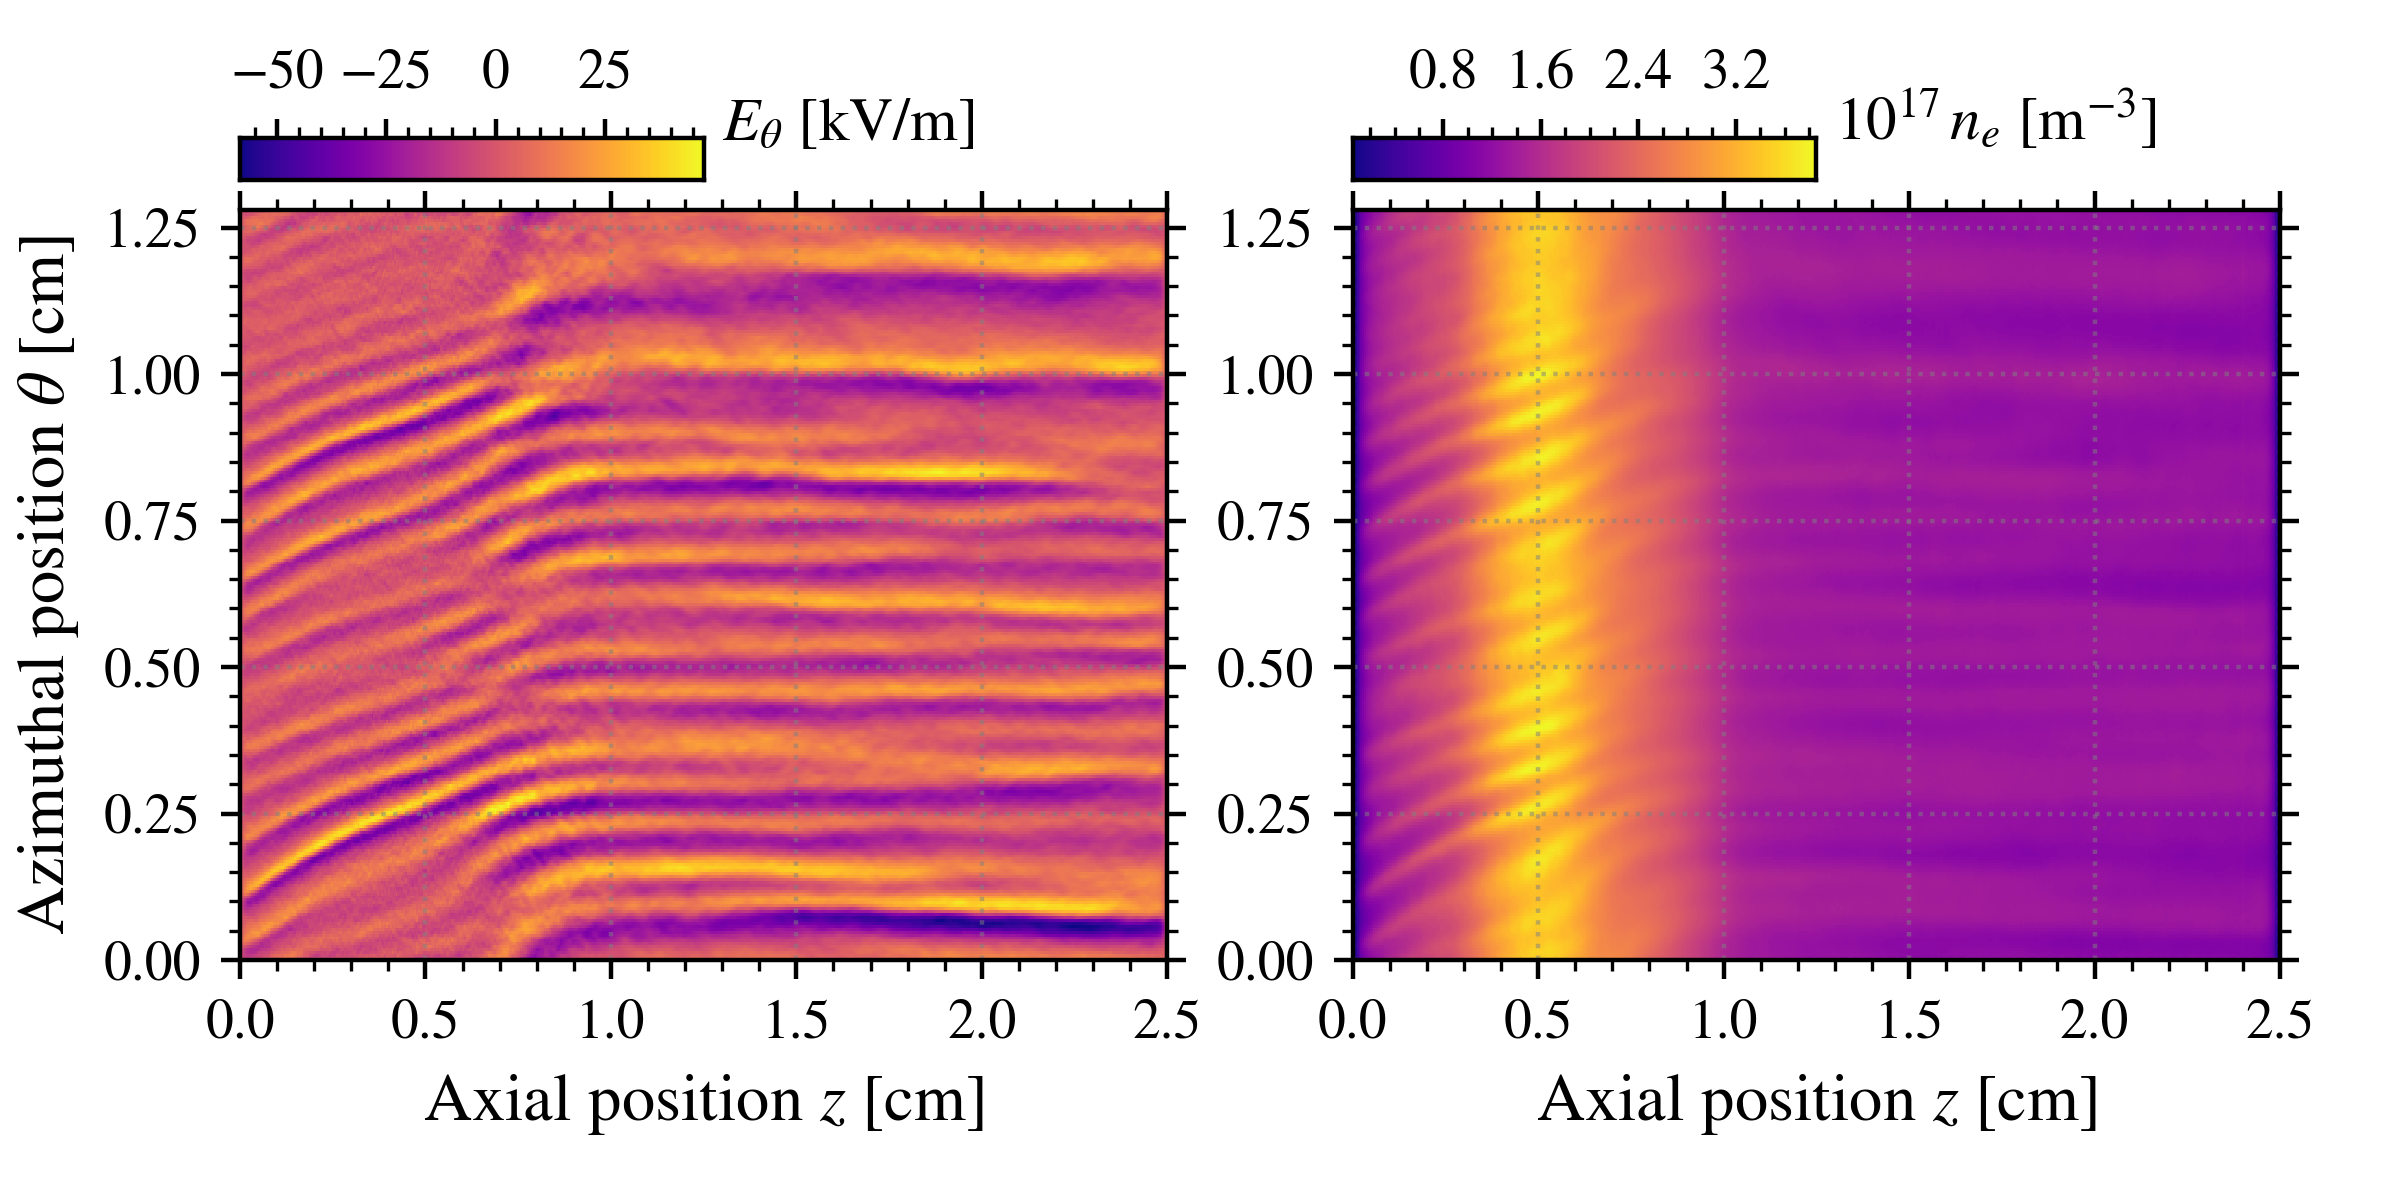
\includegraphics[width=0.9\textwidth]{Boeuf_example_t=8}
    \caption{ Axial-azimuthal distributions of (left) the azimuthal electric field $E_{\theta}$ and (right) the electron density $n_e$ at $t=8\,\micro\second$ for the test-case of Boeuf. } 
    \label{fig-overview_boeuf_neEx}
  \end{figure}

  \subsection{Boeuf test-case: Temporal evolution} \label{subsec-temp_boeuf}
  
  Since the ionization source term is constant in this test-case, a steady state is reached after a 6 or $8\micro\second$.
  \Cref{fig-boeuf-temporal} presents the temporal evolution of the mean plasma density and temperature.
  We see that when the radial direction is modeled, the density and the mean electron temperature and the radial electron temperature is reduced, as expected when increasing the losses with a constant ionization source term.


  \begin{figure}[hbt]
    \centering
    \begin{tabular}{cc}
      \subfigure{Boeuf_ne_temporal}{a}{20,20} &
      \subfigure{Boeuf_Te_temporal}{b}{20,20} \\
    \end{tabular}
    \caption{({\bf a}) temporal evolution of the mean plasma density and  ({\bf b})  temporal evolution of the  electron temperatures obtained with three different radial models for the simulation case of Boeuf. }
    \label{fig-boeuf-temporal}
  \end{figure}

  We see on \cref{fig-boeuf-temporal}.{\bf b} that the radial temperature remains constant when the radial direction is not modeled.
  This is due to the fact that the collisions are not modeled in the simulations, so that there is not momentum and energy transfer possible from the axial and azimuthal directions, and the radial direction.

  However, we know from the radial-azimuthal simulations that there is a transfer, resulting in a plasma less anisotropic than observed here.
  This aspect is discussed in \cref{subsec-MCC_boeuf,subsec-radial-heating}.
  With the radial losses, the radial temperature decreases from the initial temperature $\Te=5\,\volt$ to $\Te_R\simeq 2.2$ and $ 3.3\,\volt$ for $L_R=2$ and $3\,\centi\meter$, respectively.
  The total temperature $\Te$ shows a similar decrease with the increase of the radial losses.

  \subsection{Boeuf test-case: Axial profiles} \label{subsec-axial_boeuf}

  \Cref{fig-boeuf_axialone,fig-boeuf_axialtwo}  show the axial profile at steady-state of several plasma quantities.
  The variables are averaged in the azimuthal direction and in time between $t=8$ and $t=10\,\micro\second$.
  The results  obtained with three different radial models for the simulation case of Boeuf are overlaid.
  \cref{fig-boeuf_axialone}.{\bf a} shows the axial electric field $E_z$.
  The differences in $E_z$ are small, but we can still distinguish that the amplitude of $E_z$ is reduced with the increased radial losses.
  The electron density $n_e$ shown in \cref{fig-boeuf_axialone}.{\bf b} is almost not affected, except in for $z>1\,\centi\meter$, where the electron losses at the wall can be seen.

  \begin{figure}[hbt]
    \centering
    \begin{tabular}{cc}
      \subfigure{Boeuf_electric_field}{a}{30,22} &
      \subfigure{Boeuf_ne_axial}{b}{30,24} \\
    \end{tabular}
    \caption{Averaged axial profiles at steady state of ({\bf a}) the axial electric field $E_z$, ({\bf b}) the mean plasma density obtained with three different radial models for the simulation case of Boeuf. }
    \label{fig-boeuf_axialone}
  \end{figure}

  On the other hand, the axial electron density current $J_{e, z}$ (\cref{fig-boeuf_axialtwo}.{\bf a}) and the electron temperature (\cref{fig-boeuf_axialtwo}.{\bf b}) are significantly reduced when the radial losses are modeled.
  We see a factor of two on $J_{e, z}$ between the case $L_R=2\,\centi\meter$ and the case without losses.
  However, we have seen that the electron density is almost unaffected.
  This means that the electron axial velocity is reduced, because of the radial losses.

  \begin{figure}[hbt]
    \centering
    \begin{tabular}{cc}
      \subfigure{Boeuf_Je_axial}{a}{30,22} &
      \subfigure{Boeuf_Te_axial}{b}{25,80} \\
    \end{tabular}
    \caption{Averaged axial profile at steady state of ({\bf a})  the axial electron current density $J_{e, z}$, and ({\bf b}) the  electron temperature obtained with three different radial models for the simulation case of Boeuf. }
    \label{fig-boeuf_axialtwo}
  \end{figure}


  We see that the electron transport is highly affected.
  This is expected to be due to the reduced electron temperature, which reduces the amplitude of the instability at saturation.
  It is confirmed by the values presented in \Cref{fig-boeuf-instability}.
  \cref{fig-boeuf-instability} shows on the left the average standard deviation of the azimuthal electric field.
  It represents the amplitude of the oscillation.
  We casee that the amplitude of the instability is significantly affected by the electron radial losses.

  \begin{figure}[hbt]
    \centering
    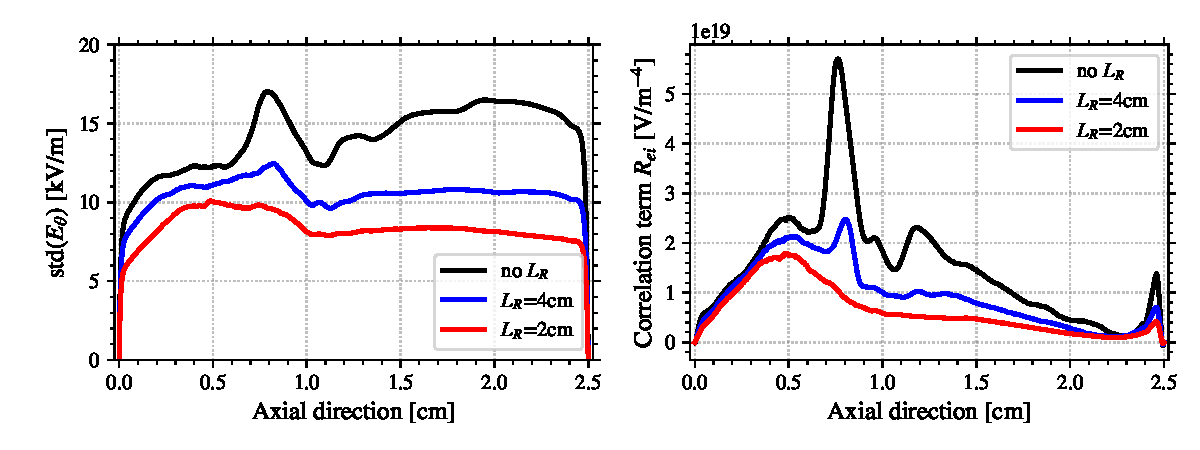
\includegraphics[width=\textwidth]{Boeuf_instability_characteristics}
    \caption{Axial profiles of the characteristics of the instability, (left) average of the standard deviation of the azimuthal electric field, (right) electron-ion friction force calculated by the correlation between $n_e$ and $\Te$.    }
    \label{fig-boeuf-instability}
  \end{figure}

  On the right panel of \cref{fig-boeuf-instability} we see the correlation term
  \begin{equation} \label{eq-rei}
    R_{ei} = < n_e E_{\theta} >
  \end{equation}
  responsible for the electron axial enhanced transport.
  Again, we see a decrease on the amplitude of $R_{ei}$ because of the reduced oscillation amplitude.


  \subsection{Boeuf test-case with collisions} \label{subsec-MCC_boeuf}
  % Script on Juno (CH-6_Boeuf)

  We have seen that because there is no collision in the test-case of Boeuf, there is no energy transfer toward the radial direction.
  Thus, we investigate here the impact of the neutrals on the electron anisotropy by modeling the collisions with the \ac{MCC} algorithm.
  We uses the same model as in the test-case of Coche, described in \cref{subsec-coche_description}.

  The xenon neutrals are injected at the anode side with density of $n_g=\sn{1}{17}\,\meter$${-3}$, an axial velocity $v_g = 200 \,\meter\per\second$ and a temperature $T_g=640\,\kelvin$.
  We model the neutral flow with the continuity and momentum conservation equation, while keeping their temperature constant.
  The ionization source term used to sustain the plasma is used as the loss term in the continuity equation.
  \Cref{fig-boeuf-neutrals} shows the neutral density and velocity obtained at steady-state.

  \begin{figure}[hbt]
    \centering
    \begin{tabular}{cc}
      \subfigure{boeuf_MCC_ng}{a}{20,20} &
      \subfigure{boeuf_MCC_vg}{b}{20,15} \\
    \end{tabular}
    \caption{Axial profile at steady-state ($t=14\,\micro\second$) of ({\bf a}) the neutral density and  ({\bf b})  the neutral axial velocity, for  simulation case of Boeuf with the electron-neutral scattering. }
    \label{fig-boeuf-neutrals}
  \end{figure}
  We see in \cref{fig-boeuf-neutrals} that the neutral density is significantly depleted because of the forced ionization source term.
  The neutral density gradient accelerates the neutrals in the axial direction by a factor of two, which reduces even more the neutral density.
  Thus, the electron-neutral scattering will be significant on the anode side of the chamber.

  \begin{figure}[hbt]
    \centering
    \begin{tabular}{cc}
      \subfigure{boeuf_mean_Te}{a}{20,20} &
      \subfigure{boeuf_mean_Tez_profile_MCC}{b}{20,15} \\
    \end{tabular}
    \caption{({\bf a}) temporal evolution of the electron kinetic energy in the three directions and  ({\bf b}) axial profile of the electron temperature at steady state obtained for the simulation case of Boeuf with the electron-neutral scattering. }
    \label{fig-boeuf-temporalMCC}
  \end{figure}

  \Cref{fig-boeuf-temporalMCC} shows the temporal evolution of the mean electron kinetic energy on the left, and on the right it shows the axial profile of the electron temperatures, decomposed on the three directions.
  We see that they is a small transfer of energy between the radial direction and the others.
  In particular, close to the anode where the gas density is high, the radial and axial temperatures decrease below the initial temperature $\Te_{, inj}=5\,\volt$.
  In contrast, at the maximum of the magnetic field where the gas density is low (and then electron neutral scattering is considered to be negligible), the radial energy increases to $\Te_R=7\,\volt$.
  However, the anisotropy stays significant, compared to the  radial-azimuthal simulations presented in \cref{ch-2}.

  \subsection{Radial heating of electrons} \label{subsec-radial-heating}
  The large anisotropy observed in \Cref{fig-boeuf-temporal,fig-boeuf-temporalMCC}, compared to the results of \cref{ch-2} might be due to the difference on neutral density.
  However, the collisions are usually neglected in \ac{HET}s compared to the instability.
  Hence, the plasma fluctuations may be responsible for the electron radial heating.

  The electron power gain is due to Joule heating
  \begin{equation} \label{eq-epower}
      \vect{P_{\rm J}} = \vect{J_e} \cdot \vect{E},
  \end{equation}
  with $\vect{J_e}$ the electron density current and $\vect{E}$ the electric field.
  \Cref{fig-epower_radialone} shows the radial profiles of the electron (and ion) current density $< J_{e, R}>$ and the radial electric field $ < E_R >$, averaged in the azimuthal direction.
  The current density increases linearly with the radial position.
  This is due to the artificial uniform injection of particles that compensates the radial losses (see \cref{sec-bidimentionnal_simulation} for more details).


  \begin{figure}[hbt]
    \centering
    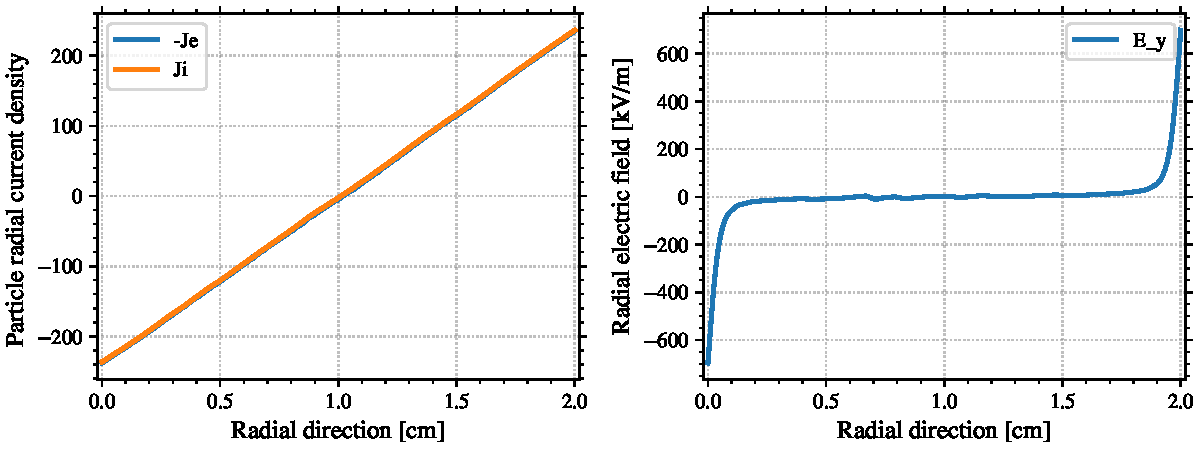
\includegraphics[width=\textwidth]{R_joule_heating_one}
    \caption{Radial profiles averaged in the azimuthal direction of (left) the electron and ion current densities and (right) radial electric field in the radial-azimuthal \ac{PIC} simulation presented in \cref{ch-2}. }
    \label{fig-epower_radialone}
  \end{figure}

  \Cref{fig-epower_radial} shows the mean Joule heating in the radial direction $\bar{P_{\rm J, R}} = < J_{e, R} E_R >$, and the product of the mean quantities $< J_{e, R}>  < E_R >$.
  The product $< J_{e, R}>  < E_R >$ is close to zero , except in the sheaths.

  \begin{figure}[hbt]
    \centering
    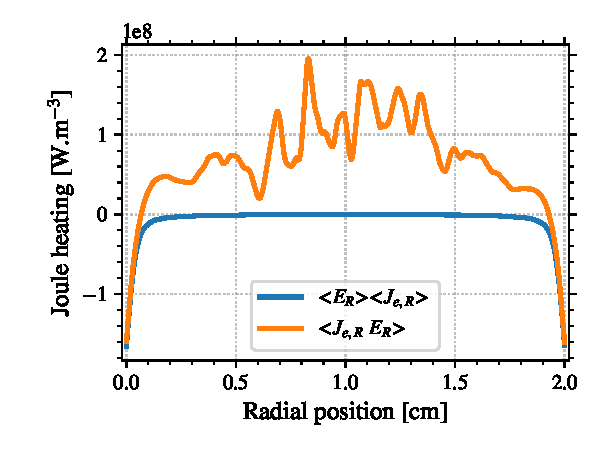
\includegraphics[width=\defaultwidth]{R_joule_heating_two}
    \caption{Electron power gain in the Radial-azimuthal }
    \label{fig-epower_radial}
  \end{figure}

  We see that the mean Joule heating $\bar{P_{\rm J, R}}$ is not zero in the center of the simulation, while the product of the mean is zero.
  Indeed, the mean electric field in the bulk is almost zero.
  This means that there is an energy transfer to the radial direction of the electrons due to the correlation between $\vect{J_e}$ and $\vect{E}$.
  For this energy transfer to be present, the radial direction needs to be resolved.

  A similar radial heating has been observed by \citet{heron2013}.
  The authors observe no heating when the instability was only perpendicular to the magnetic field, as it is in a \ac{1D} or a \ac{2D} axial-azimuthal simulation.
  However, when the direction parallel to the magnetic field is resolved, the electrons are heated, but the physical mechanism remains unclear.
  In \citet{janhunen}, the authors observe a similar radial heating of the electrons, but due to the presence of a \ac{MTSI}.
  As discussed previously, we do not observe the \ac{MTSI} in our simulation, meaning that it has to be due to another mechanism.


  \subsection{Electron azimuthal drift velocity} \label{subsec-drift}

  We showed in \cref{ch-5} that the instability growth rate is proportional to the electron azimuthal drift.
  In the radial-azimuthal simulation, the drift was only due to the $\vect{E} \times \vect{B}$ drift
  \begin{equation} \label{eq-exbdrift}
    u_{E \times B} = - \frac{E_z}{B_r}
  \end{equation}

  \Cref{fig-Jetheta_sum} shows the axial profile of the azimuthal electron mean velocity $u_{e, \theta}$ at steady-state ($t = 14\,\micro\second$) for the case without the radial losses modeled.
  The drift velocity $u_{E \times B}$ is also shown.
  We can see that the electron velocity is no more equal to the $u_{E \times B}$ drift.
  Instead, we saw in \cref{fig-boeuf_axialtwo} that the electron density presents a large axial gradient.
  This leads to the diamagnetic drift
  $$u_{\rm Dia}=\frac{\nabla_z (n_e {\rm T}_{e,z})}{n_e B_r}.$$
  The value of the diamagnetic can be seen in \cref{fig-Jetheta_sum}.


  \begin{figure}[hbt]
    \centering
    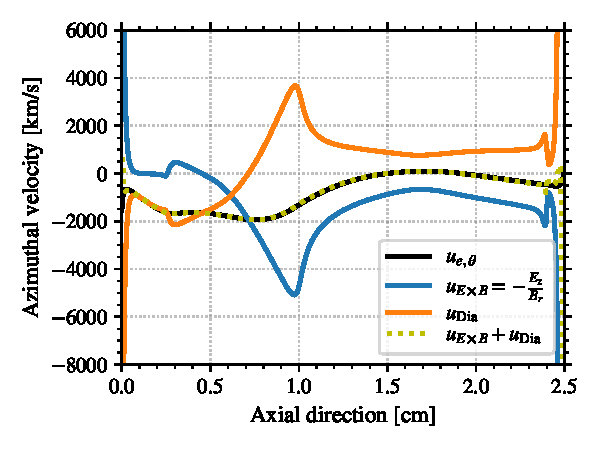
\includegraphics[width=\defaultwidth]{Boeuf_Je_x_axial_one}
    \caption{Axial profile of the electron azimuthal velocity, the $\vect{E} \times \vect{B}$ drift velocity and the diamagnetic velocity and some of the $\vect{E} \times \vect{B}$ and diamagnetic velocities at steady state for the simulation test-case of Boeuf without radial losses.}
    \label{fig-Jetheta_sum}
  \end{figure}


  We see that $u_{\rm Dia}$ is of the same order of magnitude as $u_{E \times B}$, but of the opposite sign.
  Moreover, we see that we have 
  $$ u_{e, \theta} =   u_{E \times B} + u_{\rm Dia}$$
  everywhere in the simulation domain.
  \Cref{fig-Jetheta} shows the values of $ u_{e, \theta},   u_{E \times B}$, and $u_{\rm Dia}$ for the three cases.
  We can see that the magnitude of $u_{e, \theta} $ decreases when the radial losses are present.
  However, the amplitude of both $u_{\rm Dia}$ and $u_{E \times B}$ decreases as well.

   
  \begin{figure}[hbt]
    \centering
    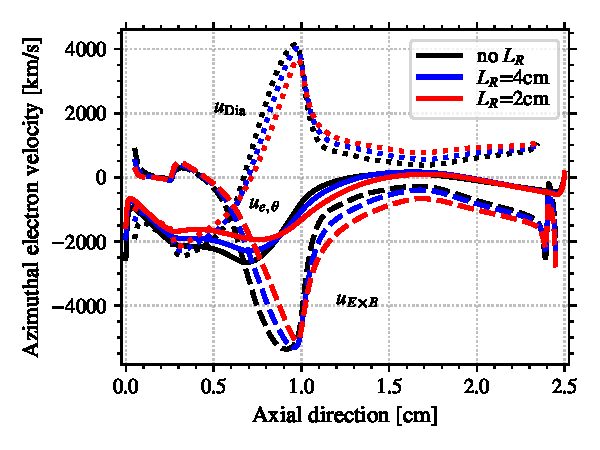
\includegraphics[width=\defaultwidth]{Boeuf_Je_x_axial}
    \caption{Axial profile of the electron azimuthal velocity, the $\vect{E} \times \vect{B}$ drift velocity and the diamagnetic velocity at steady state with three different radial models for the simulation test-case of Boeuf. The sheaths (close to the axial boundaries) are removed from the figure to ease the reading.}
    \label{fig-Jetheta}
  \end{figure}



